% CS514 final presentation -- 7 minutes, 9 main slides + backup.
% Build:  cd slides && latexmk -pdf slides.tex
% Figures come from ../figures (generated by analysis/make_figures.py).
%
% Suggested timing (total ~7:00):
%   1 Title 0:15 | 2 Motivation 0:45 | 3 Background 0:45 | 4 Method 0:50
%   5 Fig.10 0:50 | 6 Fig.11(b) 0:50 | 7 MoE bandwidth 0:55 | 8 Why 0:50
%   9 Takeaways 0:40
\documentclass[aspectratio=169,11pt]{beamer}
\usetheme[progressbar=frametitle,numbering=fraction]{metropolis}
\usepackage{booktabs}
\usepackage{graphicx}
\usepackage{tikz}
\usetikzlibrary{arrows.meta,positioning,fit,backgrounds}
\graphicspath{{../figures/}}

% ---------- colours (match the result figures) ----------
\definecolor{accent}{HTML}{E4572E}
\definecolor{cblue}{HTML}{2E6FD8}
\definecolor{cgreen}{HTML}{1FA67A}
\definecolor{cgray}{HTML}{6B7280}
\setbeamercolor{alerted text}{fg=accent}
\setbeamercolor{progress bar}{fg=accent}
\newcommand{\bignum}[1]{{\fontsize{24}{26}\selectfont\bfseries\color{accent}#1}}
\newcommand{\src}[1]{\par\vfill{\scriptsize\color{cgray}#1}}

\title{From GPT-3 to MoE: Replicating and Extending SimAI}
\subtitle{Do the paper's AI-cluster design conclusions still hold for a Mixture-of-Experts workload?}
\author{Yiheng Fan \and Ying Xiong}
\institute{CS514 Advanced Networking \quad\textbullet\quad Final Presentation}
\date{November 13, 2026}

\begin{document}

% =========================================================== 1
\maketitle

% =========================================================== 2
\begin{frame}{Motivation: SimAI guided two GPT-3 hardware decisions}
\begin{columns}[T,onlytextwidth]
\column{0.48\textwidth}
\textbf{\color{cblue}Claim 1 -- Bandwidth} \hfill {\scriptsize Fig.~10}\\[2pt]
200\,Gbit/s per GPU is \emph{enough} for H20.\\
Going 200 $\to$ 400\,Gbit/s saves only $\sim$6\% iteration time.
\column{0.48\textwidth}
\textbf{\color{cblue}Claim 2 -- Host size} \hfill {\scriptsize Fig.~11(b)}\\[2pt]
Spend bigger NVSwitch hosts on more \emph{DP}, not bigger \emph{TP}.\\
A larger TP group on a larger host can even be slower.
\end{columns}

\vspace{0.8em}
\begin{alertblock}{Our question}
Both claims come from a \textbf{dense} model.
Do they hold for \textbf{MoE}, whose all-to-all traffic depends on where the experts are placed?
\end{alertblock}

\begin{enumerate}\small
  \item \textbf{Replicate} Figs.~10 and 11(b) with the public SimAI toolchain.
  \item \textbf{Extend} the same studies to DeepSeek-V2-Lite (MoE).
\end{enumerate}
\src{X.~Wang et al., ``SimAI: Unifying Architecture Design and Performance Tuning for Large-Scale LLM Training,'' NSDI 2025.}
\end{frame}

% =========================================================== 3
\begin{frame}{Background: where each kind of traffic goes}
\begin{columns}[c,onlytextwidth]
\column{0.52\textwidth}
\centering
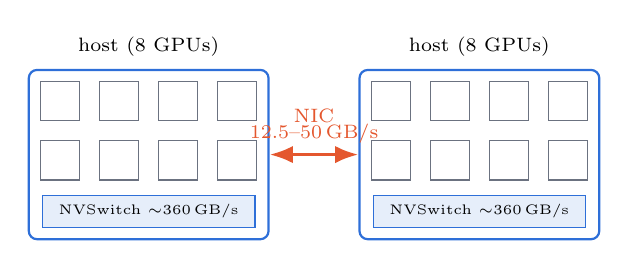
\begin{tikzpicture}[
  gpu/.style={draw=cgray,fill=white,minimum width=5mm,minimum height=5mm,inner sep=0,font=\tiny},
  host/.style={draw=cblue,thick,rounded corners=3pt,inner sep=4pt},
  lbl/.style={font=\scriptsize}]
  \foreach \h/\x in {A/0,B/4.2}{
    \foreach \i in {0,...,3}{ \node[gpu] (\h t\i) at (\x+\i*0.75,0.75) {}; }
    \foreach \i in {0,...,3}{ \node[gpu] (\h b\i) at (\x+\i*0.75,0) {}; }
    \node[draw=cblue,fill=cblue!12,minimum width=2.7cm,minimum height=3mm,font=\tiny] (\h sw) at (\x+1.125,-0.65) {NVSwitch $\sim$360\,GB/s};
    \begin{scope}[on background layer]
      \node[host,fit=(\h t0)(\h b3)(\h sw)] (\h) {};
    \end{scope}
  }
  \node[lbl,above=1pt of A] {host (8 GPUs)};
  \node[lbl,above=1pt of B] {host (8 GPUs)};
  \draw[{Latex}-{Latex},very thick,accent] (A.east) -- node[above,lbl,align=center]{NIC\\[-2pt]12.5--50\,GB/s} (B.east-|B.west);
\end{tikzpicture}

\vspace{4pt}
{\small Inside a host: fast NVSwitch.\quad Across hosts: \alert{NIC, 7--30$\times$ slower}.}

\column{0.45\textwidth}
\small
\begin{tabular}{@{}l l@{}}
\toprule
\textbf{Parallelism} & \textbf{Traffic} \\
\midrule
TP -- tensor & all-reduce, \emph{in host} \\
PP -- pipeline & point-to-point \\
DP -- data & gradient all-reduce, \emph{NIC} \\
\alert{EP -- expert} & \alert{all-to-all}, token dispatch \\
\bottomrule
\end{tabular}

\vspace{4pt}
\footnotesize
\textbf{MoE:} each token visits top-6 of 64 experts.\\
If the EP group fits in one host, all-to-all stays on NVSwitch; otherwise it crosses the NIC.
\end{columns}
\end{frame}

% =========================================================== 4
\begin{frame}{Method: public SimAI toolchain, no GPU required}
\centering
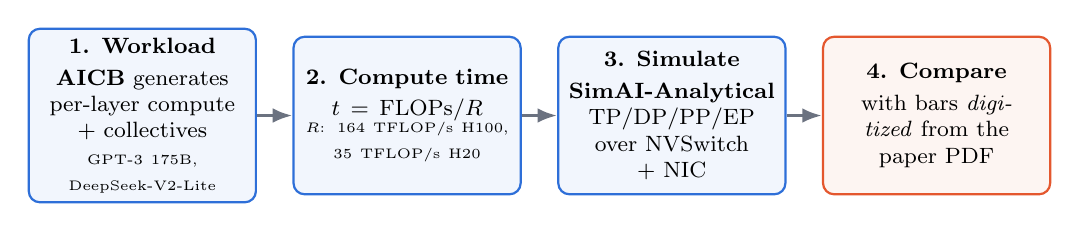
\begin{tikzpicture}[
  box/.style={draw=cblue,thick,rounded corners=4pt,fill=cblue!6,text width=2.65cm,minimum height=2.0cm,align=center,font=\footnotesize},
  arr/.style={-{Latex[length=2.5mm]},very thick,cgray}]
  \node[box] (w) {\textbf{1. Workload}\\[2pt]\textbf{AICB} generates per-layer compute + collectives\\{\tiny GPT-3 175B, DeepSeek-V2-Lite}};
  \node[box,right=0.45cm of w] (c) {\textbf{2. Compute time}\\[2pt]$t = \mathrm{FLOPs}/R$\\{\tiny $R$: 164 TFLOP/s H100,\\35 TFLOP/s H20}};
  \node[box,right=0.45cm of c] (s) {\textbf{3. Simulate}\\[2pt]\textbf{SimAI-Analytical}\\TP/DP/PP/EP over NVSwitch + NIC};
  \node[box,right=0.45cm of s,draw=accent,fill=accent!6] (p) {\textbf{4. Compare}\\[2pt]with bars \emph{digitized} from the paper PDF};
  \draw[arr] (w)--(c); \draw[arr] (c)--(s); \draw[arr] (s)--(p);
\end{tikzpicture}

\vspace{0.6em}
\begin{columns}[T,onlytextwidth]
\column{0.5\textwidth}
\small
\begin{alertblock}{One calibration point per GPU}
$R$ is fitted only to the \emph{computation} segment of the 100\,Gbit/s bar.
\textbf{Every other bar is a prediction.}
\end{alertblock}
\column{0.46\textwidth}
\footnotesize
\textbf{Setup}
\begin{itemize}\setlength\itemsep{0pt}
  \item GPT-3: TP 8 $\times$ PP 8, 1 NIC/GPU, global batch 64
  \item MoE: 64 experts, top-6, EP 8--64, on 1{,}024 and 256 GPUs
  \item Full pipeline reruns in $\sim$45\,min on a laptop CPU
\end{itemize}
\end{columns}
\end{frame}

% =========================================================== 5
\begin{frame}{Replication -- Fig.~10: bandwidth study reproduces within 0.5\%}
\begin{columns}[c,onlytextwidth]
\column{0.62\textwidth}
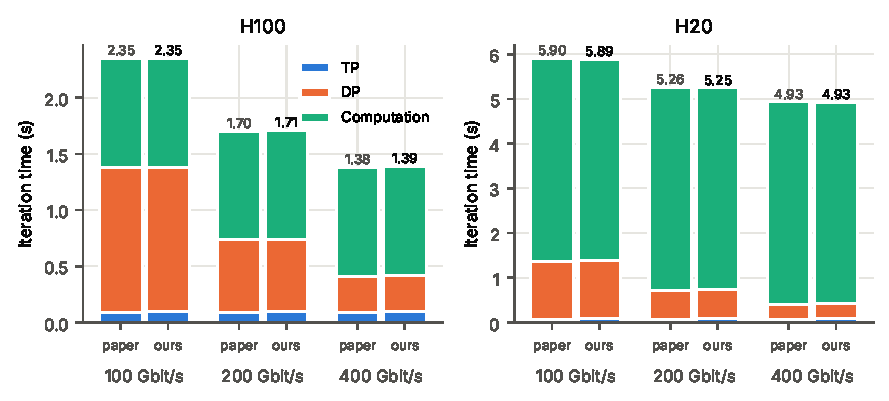
\includegraphics[width=\linewidth]{fig10_replication.pdf}
\column{0.36\textwidth}
\centering
\bignum{$<$0.5\%}\\[-2pt]
{\footnotesize max error on the four predicted bars}

\vspace{6pt}
\footnotesize
\begin{tabular}{@{}lcc@{}}
\toprule
Time saved & Paper & Ours \\
\midrule
H100, 200$\to$400 & 19\% & 18.8\% \\
H20, 100$\to$200 & 11\% & 10.9\% \\
H20, 200$\to$400 & 6\% & \textbf{6.1\%} \\
\bottomrule
\end{tabular}

\vspace{8pt}
\raggedright
\textbf{Claim 1 holds.} H20 is compute-bound, so extra bandwidth buys little.
\end{columns}
\src{GPT-3 175B, TP 8 $\times$ PP 8, one NIC per GPU.}
\end{frame}

% =========================================================== 6
\begin{frame}{Replication -- Fig.~11(b): host size reproduces only in direction}
\begin{columns}[c,onlytextwidth]
\column{0.62\textwidth}
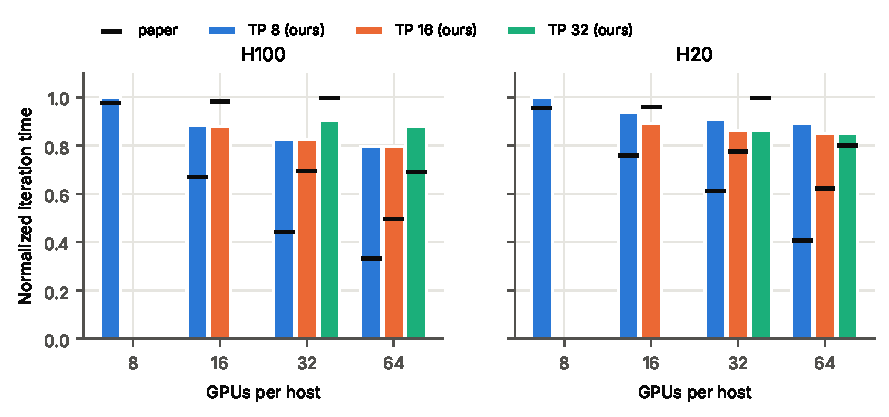
\includegraphics[width=\linewidth]{fig11b_replication.pdf}
{\scriptsize Bars: ours\quad Black ticks: paper\quad Normalized to 8-GPU host, TP 8}
\column{0.36\textwidth}
\footnotesize
\textbf{\color{cgreen}Holds:} bigger hosts are faster; TP 32 is slowest on H100.

\vspace{6pt}
\textbf{\color{accent}Gap:} the paper's gains are much larger (64-GPU host, TP 8: 0.33 vs.\ our 0.80); on H20 our TP 32 is not slower.

\vspace{6pt}
\textbf{Why:} the TP ranking appears only if per-GPU kernels stop speeding up beyond TP 8 -- an efficiency effect FLOP-based timing cannot see.
\end{columns}
\end{frame}

% =========================================================== 7
\begin{frame}{Extension -- DeepSeek-V2-Lite: MoE gets more out of extra bandwidth}
\begin{columns}[c,onlytextwidth]
\column{0.62\textwidth}
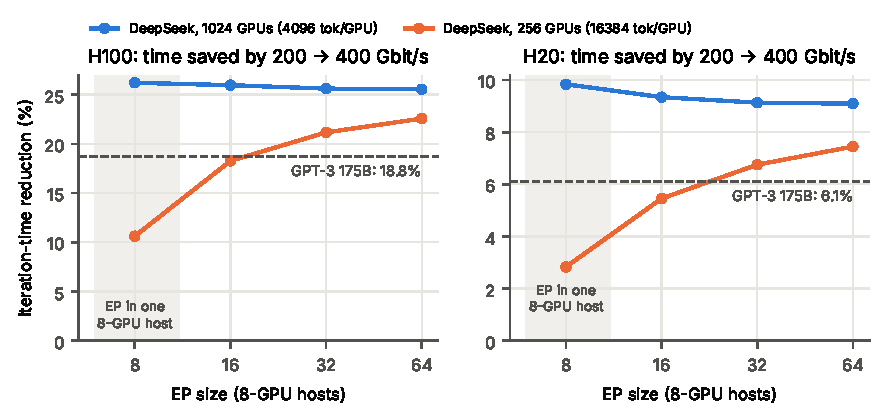
\includegraphics[width=\linewidth]{moe_bandwidth_gain.pdf}
\column{0.36\textwidth}
\centering
\bignum{9--10\%}\\[-2pt]
{\footnotesize H20 time saved by 200$\to$400\,Gbit/s\\at 4K tokens/GPU (GPT-3: 6.1\%)}

\vspace{6pt}
\raggedright\footnotesize
\begin{itemize}\setlength\itemsep{1pt}
  \item 16K tokens/GPU (256 GPUs): gain climbs \textbf{2.8\% $\to$ 7.4\%} as EP groups leave the 8-GPU host.
  \item H100: 10\% $\to$ 22\% over the same range.
  \item Rankings hold under $\pm$25\% compute time.
\end{itemize}
\end{columns}
\end{frame}

% =========================================================== 8
\begin{frame}{Why: two kinds of MoE traffic trade places}
\begin{columns}[c,onlytextwidth]
\column{0.62\textwidth}
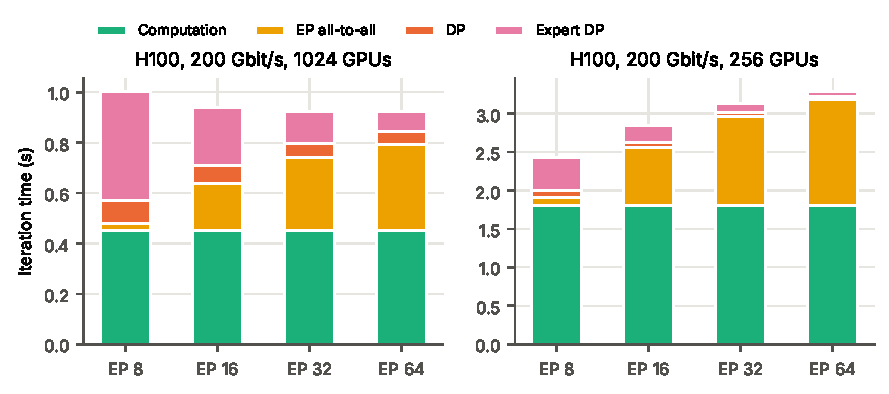
\includegraphics[width=\linewidth]{moe_breakdown.pdf}
{\scriptsize H100, 200\,Gbit/s.\quad Expert DP = gradient sync of expert parameters.}
\column{0.36\textwidth}
\footnotesize
\textbf{Small EP (8)}\\
all-to-all stays on NVSwitch, but each GPU holds 8 experts whose gradients sync \alert{over the NIC}.

\vspace{6pt}
\textbf{Large EP (64)}\\
all-to-all moves \alert{onto the NIC}, while expert-gradient traffic shrinks.

\vspace{6pt}
\textbf{Net effect}\\
1{,}024 GPUs: the two nearly cancel.\\
256 GPUs: all-to-all dominates.
\end{columns}
\end{frame}

% =========================================================== 9
\begin{frame}{Takeaways: what carries over to MoE}
\begin{enumerate}\setlength\itemsep{6pt}
  \item SimAI's bandwidth result is \textbf{reproducible} with public tools and one calibration point: within 0.5\%.
  \item ``200\,Gbit/s is enough for H20'' \textbf{still holds for MoE} when tokens per GPU are high and EP fits inside one host.
  \item Extra bandwidth is \textbf{worth more for MoE} when tokens per GPU are low or EP spans hosts; larger NVSwitch hosts help MoE more than GPT-3.
\end{enumerate}

\vspace{6pt}
\begin{block}{Limits}
\small
FLOP-based compute misses kernel efficiency (the Fig.~11(b) gap)
\textbullet\ main results assume evenly loaded experts
\textbullet\ analytical simulator: no congestion.
\end{block}
\src{Code, raw outputs and figures: \texttt{github.com/Yiheng03/cs514-ai-cluster-networking}}
\end{frame}

{\setbeamercolor{palette primary}{fg=black,bg=white}
\begin{frame}[standout]
  Thank you!\\[6pt]
  {\normalsize Questions?}
\end{frame}}

% =========================================================== backup
\appendix

\begin{frame}{Backup: host size for MoE}
\begin{columns}[c,onlytextwidth]
\column{0.62\textwidth}
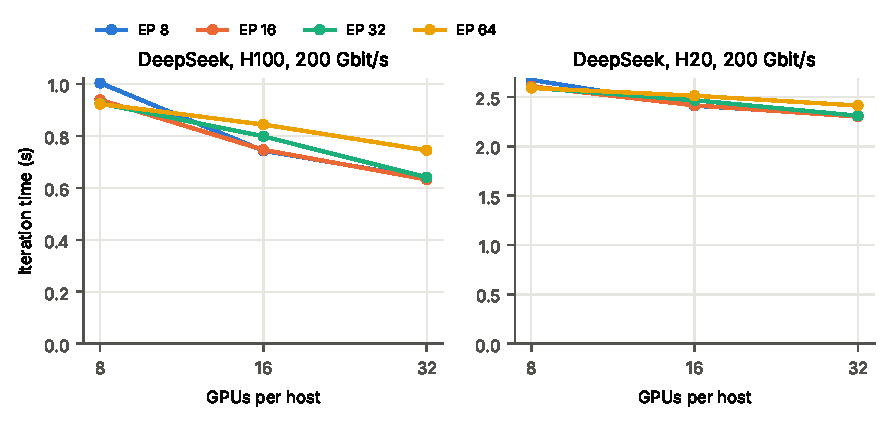
\includegraphics[width=\linewidth]{moe_hostsize.pdf}
\column{0.36\textwidth}
\footnotesize
Growing the host from 8 to 32 GPUs (1{,}024 GPUs):
\begin{itemize}\setlength\itemsep{2pt}
  \item H100, 200\,Gbit/s: $-$19\% (EP 64) to $-$37\% (EP 8).
  \item H20, 200\,Gbit/s: $-$7\% to $-$14\%.
  \item GPT-3 H20, TP 8: $-$9\%.
\end{itemize}
Adding TP to MoE (EP 16, H100) makes it slower: TP 1/2/4 = 0.94 / 1.01 / 1.15\,s, consistent with Claim 2.
\end{columns}
\end{frame}

\begin{frame}{Backup: expert load imbalance}
\begin{columns}[c,onlytextwidth]
\column{0.62\textwidth}
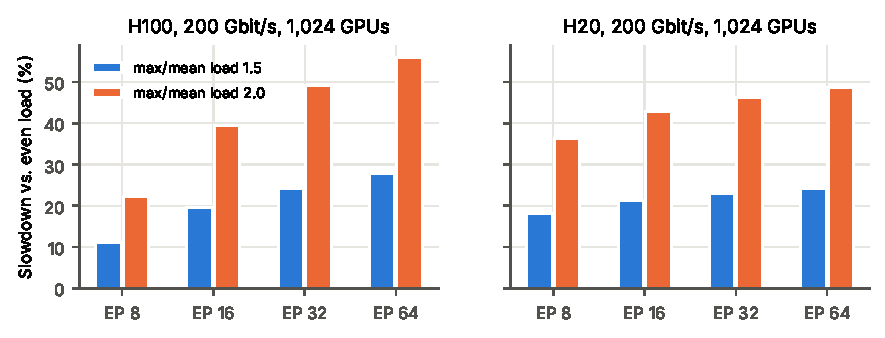
\includegraphics[width=\linewidth]{moe_skew.pdf}
\column{0.36\textwidth}
\footnotesize
Slowdown when the busiest expert receives 1.5$\times$ or 2$\times$ the mean load:
\begin{itemize}\setlength\itemsep{2pt}
  \item 1.5$\times$: +11--27\% (H100), +17--24\% (H20).
  \item 2$\times$: up to +55\% (H100, EP 64).
\end{itemize}
Skew hurts more at large EP, where the hot expert's all-to-all crosses the NIC.
\end{columns}
\end{frame}

\begin{frame}{Backup: assumptions}
\small
\begin{itemize}\setlength\itemsep{3pt}
  \item One NIC per GPU: 100/200/400\,Gbit/s = 12.5/25/50\,GB/s; NVLink 360\,GB/s (H100 and H20).
  \item GPT-3: TP 8, PP 8, seq 2048, micro-batch 1, \textbf{global batch 64} (not in the paper; chosen to match the paper's TP time; 32--256 tested).
  \item Fig.~11(b) bandwidth: 400\,Gbit/s (H100) / 200\,Gbit/s (H20), the production designs.
  \item Distributed-optimizer parameter all-gather placed in the DP group.
  \item DeepSeek-V2-Lite with its published hidden size 2048 (AICB's preset uses 10944); small AICB patch to build MoE workloads without a GPU.
  \item Memory check: model state is 9--19\,GB/GPU for every configuration, so all fit in 80\,GB (H100) / 96\,GB (H20).
  \item SimAI pinned at commit \texttt{a57d765}, AICB at \texttt{23eec3c}.
\end{itemize}
\end{frame}

\end{document}
